\begin{figure}[t]
\centering
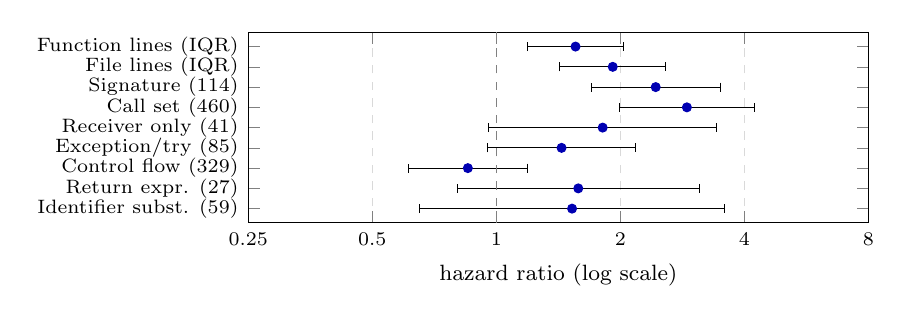
\begin{tikzpicture}
\begin{axis}[width=0.78\columnwidth,height=4.0cm,xmode=log,log basis x=2,xmin=0.25,xmax=8,xtick={0.25,0.5,1,2,4,8},
  xticklabels={0.25,0.5,1,2,4,8},ytick={9,8,7,6,5,4,3,2,1},yticklabels={{Function lines (IQR)},{File lines (IQR)},{Signature (114)},{Call set (460)},{Receiver only (41)},{Exception/try (85)},{Control flow (329)},{Return expr. (27)},{Identifier subst. (59)}},ymin=0.3,ymax=9.7,
  y tick label style={font=\scriptsize},x tick label style={font=\scriptsize},xlabel={hazard ratio (log scale)},label style={font=\footnotesize},
  xmajorgrids,grid style={dashed,gray!30}]
\addplot[only marks,mark=*,mark size=1.6pt,blue!70!black,error bars/.cd,x dir=both,x explicit,error bar style={black}] coordinates {(1.557,9) -= (0.364,0) += (0.475,0) (1.917,8) -= (0.490,0) += (0.659,0) (2.437,7) -= (0.736,0) += (1.055,0) (2.901,6) -= (0.913,0) += (1.333,0) (1.812,5) -= (0.855,0) += (1.619,0) (1.440,4) -= (0.488,0) += (0.738,0) (0.853,3) -= (0.242,0) += (0.339,0) (1.581,2) -= (0.777,0) += (1.529,0) (1.527,1) -= (0.875,0) += (2.048,0)};
\draw[gray,dashed] (axis cs:1,0.3) -- (axis cs:1,9.7);
\end{axis}
\end{tikzpicture}
\caption{Hazard ratios with 95\% CIs (cloglog model): churn per inter-quartile range; change types (touches with the flag) vs.\ other local edits.}
\label{fig:forest}
\end{figure}
